% These slides originally from Paul Goldsmith-Pinkham: https://github.com/paulgp

\documentclass[11pt]{article}
\usepackage[top=0.8in, bottom=0.78in, left=0.87in, right=0.87in]{geometry}
\usepackage{setspace}
\usepackage[T1]{fontenc}
\usepackage{times}
\usepackage{booktabs}
\usepackage{rotating}
\usepackage{graphicx}
\usepackage[section]{placeins} %Placeins.sty keeps floats `in their place', preventing them from floating past a "\FloatBarrier" command into another section.  To use it, declare "\usepackage{placeins}" and insert "\FloatBarrier" at places that floats should not move past, perhaps at every "\section".  
\usepackage[large, bf]{caption}
\usepackage[FIGTOPCAP]{subfigure}
\usepackage{pdfpages}
\usepackage{palatino}
\usepackage{pdflscape}
\usepackage{textcomp}
\usepackage{longtable}
\usepackage{nicefrac}
\usepackage{adjustbox}	% to adjust the size of objects to fit into a page
\usepackage[hyphens]{url}

\usepackage{natbib}
\bibpunct{(}{)}{;}{a}{,}{,}

\def\citeapos#1{\citeauthor{#1}'s (\citeyear{#1})}

%zero spacing between references
%\usepackage{bibspacing}
%\setlength{\bibspacing}{\baselineskip}

%%-----------------------------------------------------------------
%%Header
%\usepackage{fancyhdr}
%\fancyhf{}
%\fancyhead[C]{\textit{Preliminary and Incomplete}}
%\fancyfoot[C]{\thepage}
%\renewcommand\headrulewidth{0pt}
%\pagestyle{fancy}
%%-----------------------------------------------------------------

%\onehalfspacing
\doublespacing

\usepackage{amsmath, amsfonts, amssymb, amsthm}

%\usepackage{mathpazo} %Use Palotino fonts
\parskip 0ex  %Vertical distance between paragraphs, in "ex"s
\parindent 20pt

%\usepackage{harvard}
%\bibliographystyle{apsr}
%\bibliographystyle{dcu}

\usepackage[pdftex]{hyperref}
\hypersetup{colorlinks, citecolor=blue, filecolor=blue, linkcolor=blue, urlcolor=blue}

\newtheorem{theorem}{Theorem}
\newtheorem{lemma}{Lemma}
\newtheorem{proposition}{Proposition}
\newtheorem{corollary}{Corollary}
\newtheorem{prediction}{Prediction}
\newtheorem{case}{Special Case}

\newenvironment{proofAlt}[1][Proof]{\begin{trivlist}
\item[\hskip \labelsep {\bfseries #1}]}{\end{trivlist}}
\newenvironment{definition}[1][Definition]{\begin{trivlist}
\item[\hskip \labelsep {\bfseries #1}]}{\end{trivlist}}
\newenvironment{example}[1][Example]{\begin{trivlist}
\item[\hskip \labelsep {\bfseries #1}]}{\end{trivlist}}

\newenvironment{remark}[1][Remark]{\begin{trivlist}
\item[\hskip \labelsep {\bfseries #1}]}{\end{trivlist}}
\def\urltilda{\kern -.15em\lower .7ex\hbox{\~{}}\kern .04em}

\renewcommand{\thesubfigure}{(\Alph{subfigure})}

%%%%%%%%%%%%%%%%%%%%%%%%%%%%%%%%%%
% SPACING
%%%%%%%%%%%%%%%%%%%%%%%%%%%%%%%%%%

\usepackage{titlesec}

\titlespacing*{\section}{0pt}{1.5ex plus 1ex minus .2ex}{0.8ex plus .2ex}
\titlespacing*{\subsection}{0pt}{1.2ex plus 1ex minus .2ex}{0.8ex plus .2ex}
% Decimal align 
\usepackage{dcolumn}
\newcolumntype{d}[0]{D{.}{.}{5}}

\usepackage{graphicx}
\graphicspath{{../../output/}}
\usepackage[]{epstopdf}
% This adds the output directory to the inputs function (code outputs are latex inputs!) so you don't have to use a relative path each time
\makeatletter
\providecommand*{\input@path}{}
\g@addto@macro\input@path{{../../output/}}% append
\makeatother


\usepackage[space]{grffile}

 
\title{\textbf{\LARGE{PAPER TITLE}}\thanks{First version: DATE. This version: \today.  ACKNOWLEDGEMENTS HERE}}

\author{
	AUTHOR 1\thanks{UNIVERSITY 1. Email: \href{mailto:author@address.com}{author@address.com}} \and
	AUTHOR 2\thanks{UNIVERSITY 2. Email: \href{mailto:author@address.com}{author@address.com}} \and 
	AUTHOR 3\thanks{UNIVERSITY 3. Email: \href{mailto:author@address.com}{author@address.com}} \and 
	AUTHOR 4\thanks{INSTITUTION 1. Email: \href{mailto:author@address.com}{author@address.com}} 
	}
			
\date{\today}

\begin{document}

\maketitle
\thispagestyle{empty} 
\setcounter{page}{0}

\begin{abstract}
ABSTRACT HERE

\end{abstract}


	  
%%%%%%%%%%%%%%%%%%%%%%%%%%%%%%%%%
% Text
%%%%%%%%%%%%%%%%%%%%%%%%%%%%%%%%%
	
\clearpage

The model is:
$$
\begin{aligned} 
	\vec{y}_t & = \Gamma \vec{f}_t + \vec{u}_t \\ 
        \vec{f}_t & = A_1 \vec{f}_{t-1} + A_2\vec{f}_{t-2} + \Xi_t \quad \quad \Xi_t \thicksim \mathcal{N}(0,I)\\ 
	 \vec{u}_t  & = B_1 \vec{u}_{t-1} + B_2\vec{u}_{t-2} + \Phi_t \quad \quad \Phi_t \thicksim \mathcal{N}(0,\Sigma)
\end{aligned} 
$$
where capital Greek and Latin characters represent matrices, arrows over characters denote vectors, and it is assumed that the different components of the `innovations' in the error updating equation are uncorrelated so that $ \Sigma $ is a diagonal matrix. The model has one unobserved factor that follows an AR(2), and the errors similarly follow an AR(2).

\begin{center}
\begin{tabular}{lclc}
\toprule
\textbf{Dep. Variable:}          & ['emp', 'gdp', 'hhc', 'iop', 'ios']  & \textbf{  No. Observations:  } &                  349                   \\
\textbf{Model:}                  &  DynamicFactor(factors=1, order=2)   & \textbf{  Log Likelihood     } &               -1388.052                \\
\textbf{}                        &            + AR(2) errors            & \textbf{  AIC                } &                2820.103                \\
\textbf{Date:}                   &           Tue, 25 Jun 2019           & \textbf{  BIC                } &                2904.915                \\
\textbf{Time:}                   &               16:20:54               & \textbf{  HQIC               } &                2853.865                \\
\textbf{Sample:}                 &              04-30-1990              & \textbf{                     } &                                        \\
\textbf{}                        &             - 04-30-2019             & \textbf{                     } &                                        \\
\bottomrule
\end{tabular}
\begin{tabular}{lcccccc}
                          & \textbf{coef} & \textbf{std err} & \textbf{z} & \textbf{P$>$$|$z$|$} & \textbf{[0.025} & \textbf{0.975]}  \\
\midrule
\textbf{loading.f1.emp}   &       0.9011  &        0.156     &     5.772  &         0.000        &        0.595    &        1.207     \\
\textbf{loading.f1.gdp}   &       0.2574  &        0.015     &    17.045  &         0.000        &        0.228    &        0.287     \\
\textbf{loading.f1.hhc}   &       0.0004  &        0.022     &     0.017  &         0.986        &       -0.042    &        0.043     \\
\textbf{loading.f1.iop}   &       0.0675  &        0.035     &     1.936  &         0.053        &       -0.001    &        0.136     \\
\textbf{loading.f1.ios}   &       0.6151  &        0.031     &    19.841  &         0.000        &        0.554    &        0.676     \\
\textbf{sigma2.emp}       &       2.1402  &        0.285     &     7.512  &         0.000        &        1.582    &        2.699     \\
\textbf{sigma2.gdp}       &       0.0338  &        0.002     &    18.548  &         0.000        &        0.030    &        0.037     \\
\textbf{sigma2.hhc}       &       0.1712  &        0.010     &    17.204  &         0.000        &        0.152    &        0.191     \\
\textbf{sigma2.iop}       &       0.7666  &        0.066     &    11.562  &         0.000        &        0.637    &        0.897     \\
\textbf{sigma2.ios}       &       0.0033  &        0.003     &     0.962  &         0.336        &       -0.003    &        0.010     \\
\textbf{L1.f1.f1}         &       0.7777  &        0.134     &     5.788  &         0.000        &        0.514    &        1.041     \\
\textbf{L2.f1.f1}         &      -0.0798  &        0.136     &    -0.585  &         0.559        &       -0.347    &        0.188     \\
\textbf{L1.e(emp).e(emp)} &       0.8493  &        0.089     &     9.506  &         0.000        &        0.674    &        1.024     \\
\textbf{L2.e(emp).e(emp)} &      -0.0614  &        0.091     &    -0.677  &         0.498        &       -0.239    &        0.116     \\
\textbf{L1.e(gdp).e(gdp)} &       1.1448  &        0.092     &    12.491  &         0.000        &        0.965    &        1.324     \\
\textbf{L2.e(gdp).e(gdp)} &      -0.1988  &        0.093     &    -2.133  &         0.033        &       -0.381    &       -0.016     \\
\textbf{L1.e(hhc).e(hhc)} &       1.0495  &        0.139     &     7.564  &         0.000        &        0.778    &        1.321     \\
\textbf{L2.e(hhc).e(hhc)} &      -0.1598  &        0.135     &    -1.183  &         0.237        &       -0.424    &        0.105     \\
\textbf{L1.e(iop).e(iop)} &      -0.3713  &        0.081     &    -4.606  &         0.000        &       -0.529    &       -0.213     \\
\textbf{L2.e(iop).e(iop)} &       0.4494  &        0.066     &     6.787  &         0.000        &        0.320    &        0.579     \\
\textbf{L1.e(ios).e(ios)} &       0.1681  &        0.108     &     1.550  &         0.121        &       -0.045    &        0.381     \\
\textbf{L2.e(ios).e(ios)} &       0.8311  &        0.109     &     7.593  &         0.000        &        0.617    &        1.046     \\
\bottomrule
\end{tabular}
\begin{tabular}{lclc}
\textbf{Ljung-Box (Q):}          & 119.62, 57.45, 175.67, 118.54, 59.89 & \textbf{  Jarque-Bera (JB):  } & 4.71, 732.01, 1454.72, 103.47, 424.67  \\
\textbf{Prob(Q):}                &     0.00, 0.04, 0.00, 0.00, 0.02     & \textbf{  Prob(JB):          } &      0.10, 0.00, 0.00, 0.00, 0.00      \\
\textbf{Heteroskedasticity (H):} &     2.51, 0.77, 0.97, 1.50, 0.38     & \textbf{  Skew:              } &    -0.07, 0.06, 0.10, -0.37, -0.00     \\
\textbf{Prob(H) (two-sided):}    &     0.00, 0.15, 0.89, 0.03, 0.00     & \textbf{  Kurtosis:          } &     3.55, 10.09, 13.00, 5.56, 8.40     \\
\bottomrule
\end{tabular}
%\caption{Statespace Model Results}
\end{center}

Warnings: \newline
 [1] Covariance matrix calculated using the outer product of gradients (complex-step).
\begin{figure}[h]
	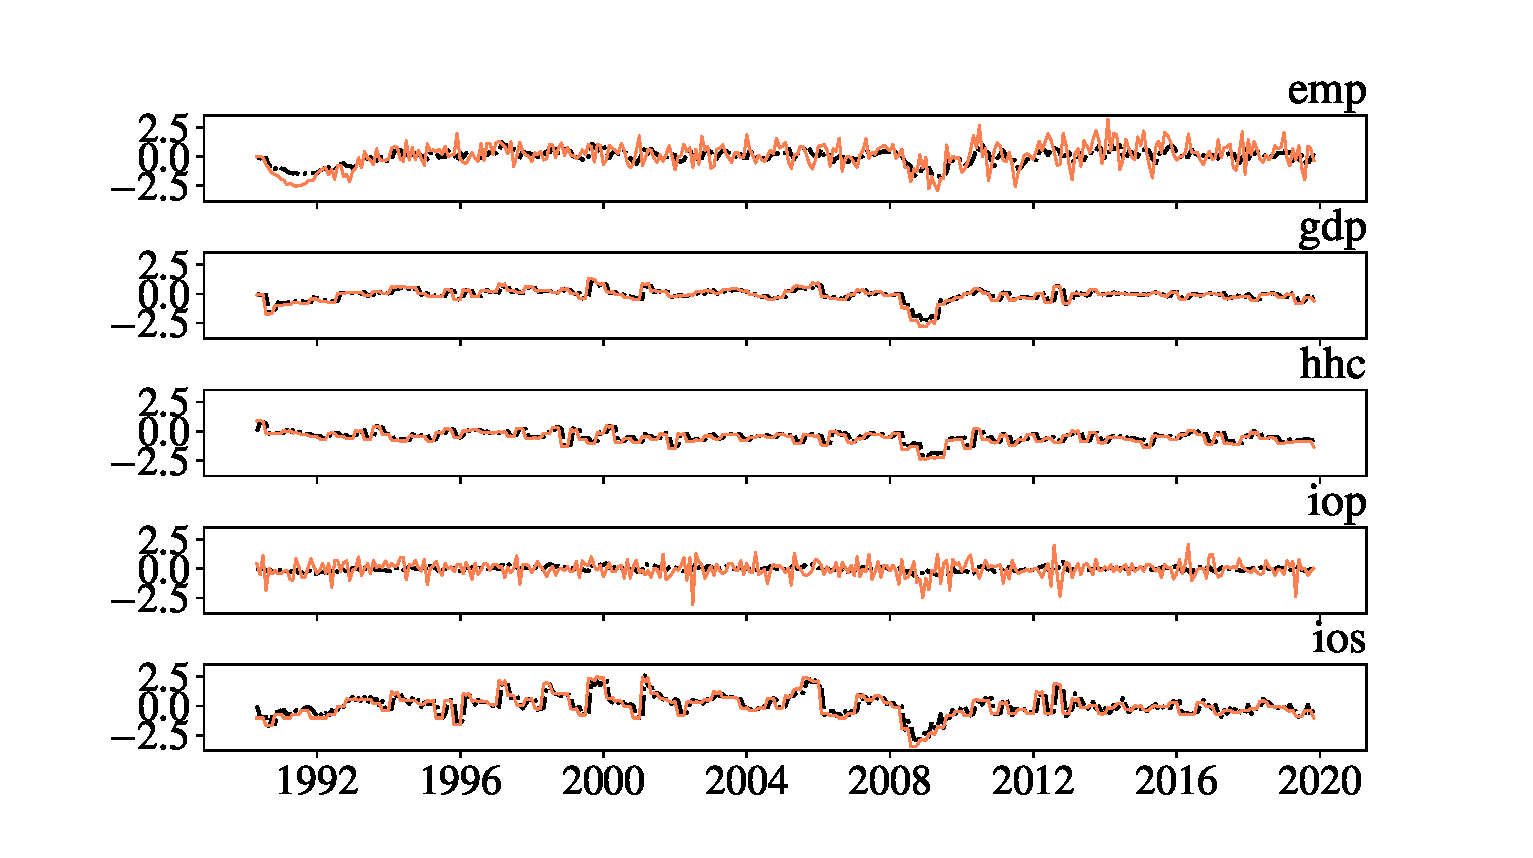
\includegraphics[width=\textwidth]{fcasts.eps} 
	\caption{Example figure. \label{fig:example}}
\end{figure}

\begin{figure}[h]
	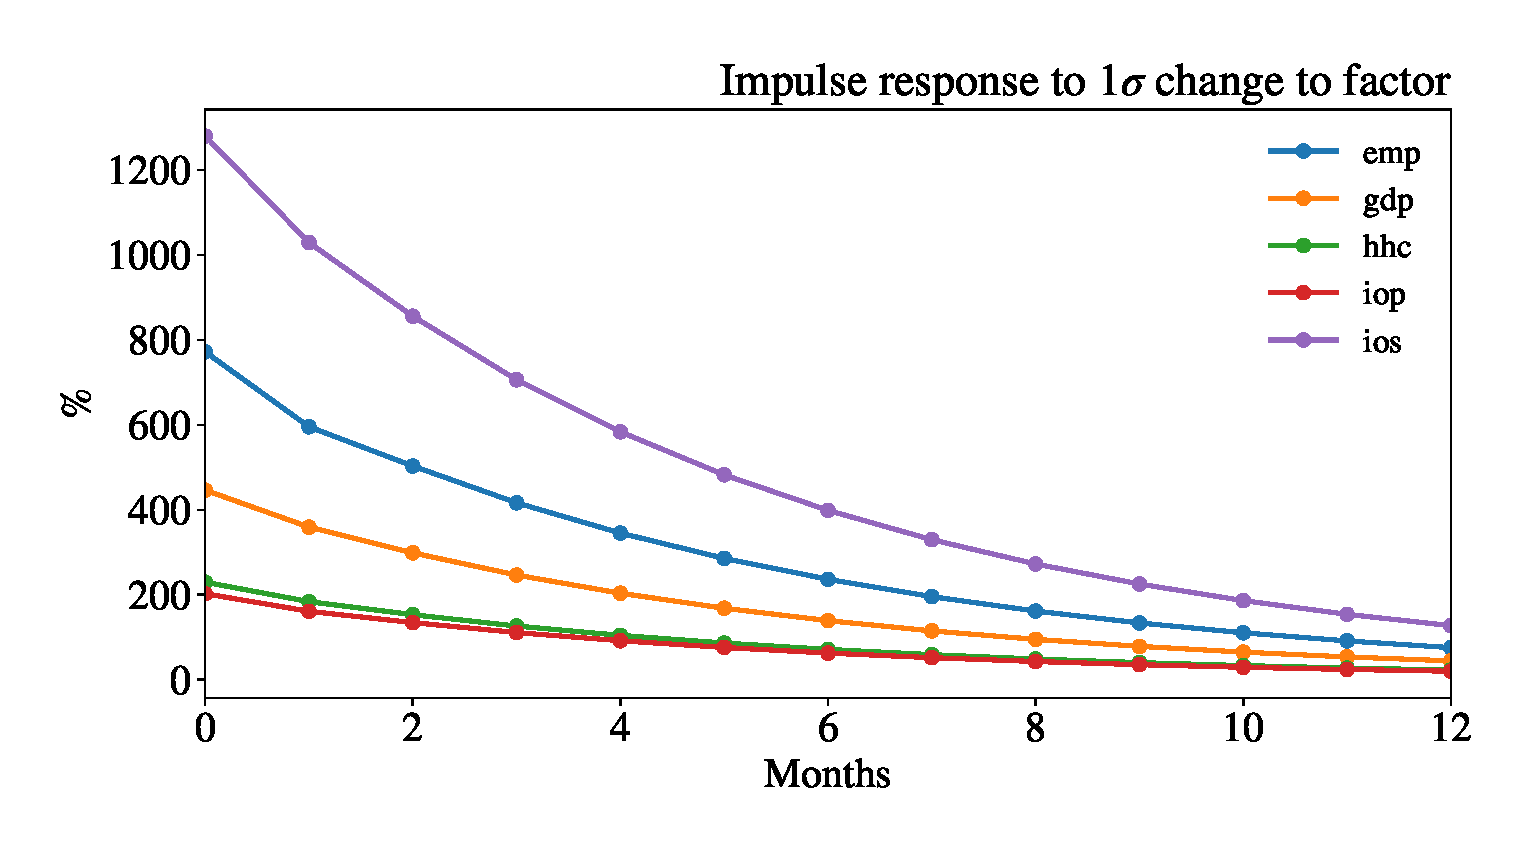
\includegraphics[width=\textwidth]{df_irfs.eps} 
	\caption{Example figure. \label{fig:example}}
\end{figure}

\newpage
\singlespacing 
\bibliographystyle{aea}
%\bibliography{bibliography.bib}

\onehalfspacing

%%%%%%%%%%%%%%%%%%%%%%%%%%%%%%%%%%
%%Figures and tables
%%%%%%%%%%%%%%%%%%%%%%%%%%%%%%%%%%

%\input{Figures.tex}
%\input{Tables.tex}

%%%%%%%%%%%%%%%%%%%%%%%%%%%%%%%%%
%Appendices
%%%%%%%%%%%%%%%%%%%%%%%%%%%%%%%%%

\clearpage  
\appendix

\renewcommand{\thefigure}{A\arabic{figure}}
\setcounter{figure}{0}

\renewcommand{\thetable}{A\arabic{table}}
\setcounter{table}{0}


\clearpage
\begin{center}
\vspace{-1.8cm}{\LARGE \textbf{PAPER TITLE}}\medskip \\
	\Large \textbf{Online Appendix} \bigskip \\
\large AUTHOR NAME 1 \hspace{0.3cm} AUTHOR NAME 2 \hspace{0.3cm} AUTHOR NAME 3 \hspace{0.3cm} AUTHOR NAME 4 \bigskip
	
\end{center}


%\input{Appendix_text.tex}

%\clearpage
%\input{Appendix_figures.tex}

%\clearpage
%\input{Appendix_tables.tex}




\end{document}
